\hypertarget{seccion:IniciarSesion}{\vspace{1pt}}
\section{Marco Teórico}

\subsection{Big Data}
El término Big Data se refiere a cantidades enormes de información, por ejemplo, la cantidad de información que se produce todos los días con el uso de una red social como Facebook, o la cantidad de datos que producen computadoras y dispositivos electrónicos que se auto monitorean mediante sensores. Esos volúmenes masivos de datos pueden ser utilizados para extraer conocimiento de ellos, y posteriormente atacar problemas que no sería posible resolver sin el Big Data.\cite{bigDataDef}

\subsubsection{Las 3 Vs del Big Data}
Al ser el Big Data un concepto emergente y relativamente nuevo, se han tenido ciertas dificultades para definirlo de manera uniforme. Debido a las dimensiones de todo lo que conlleva entender Big Data, resultó conveniente entre los estudiosos del tema definir y acentuar las magnitudes que lo definen. Estas magnitudes se conocen como las 3 Vs del Big Data.

\begin{enumerate}
	\item \textbf{Volumen:} Con Big Data, se tendrán que procesar enormes volúmenes de información. Este punto es importante ya que el crecimiento de la nececidad de almacenamiento de datos en el mundo moderno, crece de forma exponencial.\cite{bigDataDef}
	\item \textbf{Velocidad:} Usando Big Data, se abre la posibilidad de acceso y flujo de datos a velocidades que no se podrían conseguir de manera convencional.\cite{bigDataDef}
	\item \textbf{Variedad:} Procesamiento de datos de naturaleza heterogénea, es decir, múltiples tipos de datos.\cite{bigDataDef}
\end{enumerate}

\subsubsection{Casos de uso del Big Data}

\begin{UClist}
	\UCli \textbf{Desarrollo de productos:} Compañías como Netflix y Procter \& Gamble utilizan el Big Data para anticiparse a la demanda de los consumidores de sus productos. Utilizan modelos predictivos para sus nuevos productos clasificando atributos clave de sus anteriores productos modelando las relaciones entre esos atributos.\cite{bigUso}\\
	\UCli \textbf{Mantenimiento predictivo:} Se pueden predecir fallas mecánicas en maquinaria que de otra forma quedarían fácilmente ignoradas. Mejorando así ampliamente la calidad y el costo del mantenimiento de dichos equipos.\cite{bigUso}\\
	\UCli \textbf{Experiencia de usuario:} El uso de Big Data permite recopilar toda la información sobre el usuario y utilizarla a favor de su experiencia en un sitio o aplicación. Por ejemplo, sus búsquedas frecuentes, los sitios que visita, etc. Para de esta manera empezar a hacerle ofertas o anuncios personalizados, según sus intereses particulares.\cite{bigUso}\\
	\UCli \textbf{Machine Learning:} Actualmente el machine learning es un área de mucho auge, ya que permite entrenar a las computadoras mediante conjuntos de datos de entrenamiento en lugar de programarlas. El Big Data facilita esa tarea.\cite{bigUso}\\
\end{UClist}

\subsection{Minería de datos}
La minería de datos es el proceso de generar conocimiento a partir de un conjunto de información de gran tamaño. Para generar ese conocimiento se utilizan diferentes técnicas de análisis que detectan patrones y tendencias en la información que se está procesando. Si se intentara utilizar algún método de análisis tradicional, sería muy complicado o incluso imposible a veces encontrar patrones y tendencias útiles, ya que es muy probable que dentro de los datos existan relaciones muy complejas o simplemente la cantidad de datos sea demasiado grande.\cite{mineriaDef}\\

La minería de datos puede utilizarse en escenarios como los que se enuncian a continuación: \\
\begin{UClist}
	\UCli \textbf{Pronóstico:} Predicción de datos y eventos que vendrán a futuro a partir del comportamiento de conjuntos de datos que se tienen en el presente. Por ejemplo, predicción de ventas y tendencias de compra.\cite{mineriaEsc}
	\UCli \textbf{Riesgo y probabilidad:} Es un escenario muy común dentro de los negocios de Bussiness Intelligence. Por ejemplo, se llega a utilizar para encontrar puntos de equilibrio probable para escenarios de riesgo.
	Elección de los mejores clientes para la distribución de correo directo, determinación del punto de equilibrio probable para los escenarios de riesgo, y asignación de probabilidades a diagnósticos y otros resultados.\cite{mineriaEsc}
	\UCli \textbf{Recomendaciones:} Muy utilizado en sistemas como MercadoLibre o Amazon, en módulos que toman la información de búsqueda de cada usuario, la procesan y le arrojan recomendaciones de productos o servicios.\cite{mineriaEsc}
	\UCli \textbf{Búsqueda de secuencias:} Al igual que el escenario de \textbf{recomendaciones}, se utiliza mucho en sistemas de venta de artículos por internet. Se analiza el orden de los artículos que se meten a un carrito de compra para poder hacer predicciones útiles y generar conocimiento.\cite{mineriaEsc}
	\UCli \textbf{Agrupación:} Clasificación de los elementos de un conjunto de información para el posterior análisis de sus afinidades.\cite{mineriaEsc}
\end{UClist}

\subsection{Árboles de decisión}
Un árbol de decisión es un modelo de predicción que apoya al proceso de toma de decisiones. Esta herramienta tiene un campo de aplicación extremadamente amplio, pudiendo ir desde el área de finanzas hasta el área del aprendizaje de máquina. A partir de un conjunto de datos de entrada, se construyen los caminos, dentro del árbol, que llevarán a cada una de las decisiones posibles.\cite{arbolesDes}\\

Los árboles de decisión están formados por los siguientes elementos:\\

\begin{enumerate}
	\item \textbf{Nodos:} Un nodo es un punto del proceso en el que de acuerdo a ciertas condiciones o decisiones se redefine el rumbo del camino. Existen dos tipos de nodo\cite{arbolPartes}:
	\begin{enumerate}
		\item \textbf{Nodo de decisión:} Es un nodo en el cual se toma una decisión consciente de acuerdo a las necesidades del problema en cuestión. Estos nodos se representan con un cuadrado.
		\item \textbf{Nodo de incertidumbre: } Es un nodo en el que actúan las probabilidades y la heurística para definir el rumbo que tomará el camino que se hará dentro del árbol. Estos nodos se representan con un círculo
	\end{enumerate}
	\item \textbf{Ramas:} Una rama es una de las respuestas o acciones que se toman a partir de la pregunta o escenario que se presentó en un nodo del cual salió esa rama. Una rama es el camino a otro nodo o escenario resultado de la decisión o evento que definió la rama. Este elemento se representa con una línea\cite{arbolPartes}.
	\item \textbf{Hojas:} Son escenarios finales, ya clasificados. No tienen ramificaciones, y son el resultado final de seguir un camino de decisiones, acciones y probabilidades. Este elemento se representa con un triángulo\cite{arbolPartes}.
\end{enumerate}

\begin{figure}[!htbp]
	\hypertarget{fig:arbol-decision-ejemplo}{\hspace{1pt}}
	\begin{center}
		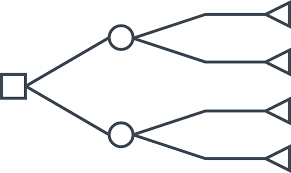
\includegraphics[height=0.3\textheight]{capitulo2/images/arbol-decision-ejemplo.png}
		\caption{Representación general de un árbol de decisión}
		\label{fig:arbol-decision-ejemplo}
	\end{center}
\end{figure}

% \newpage
\subsection{ID3 (Iterative Dichotomiser 3)} \label{id3}

El algoritmo ID3 es uno de los algoritmos que utilizan árboles de decisión más populares. ID3 genera un árbol a partir de un conjunto de datos llamado \textbf{tabla de inducción}. Es útil para hacer toma de decisiones en escenarios binarios, es decir, que tienen 2 posibilidades finales.\cite{id3}\\

El resultado de la ejecución de este algoritmo puede expresarse como un conjunto de reglas \textbf{\textit{si-entonces}}.

\subsubsection{Entropía}
La entropía es la medida de la aleatoriedad. En otras palabras, la medidad e la impredictibilidad. La entropía es más alta cuando todos los eventos posibles en un escenario son igualmente probables, por ejemplo, al tirar una moneda al aire, se tiene 50\% de probabilidad de que caiga cara y 50\% de probabilidad de que caiga cruz, por lo que la entropía es de 1. Este parámetro comienca a decrecer cuando hay una probabilidad o probabilidades que parezcan aplastantes sobre las otras. Las fórmulas para calcular la entropía y la ganancia son las siguiente:\\

\begin{figure}[!htbp]
	\hypertarget{fig:formula-entropia}{\hspace{1pt}}
	\begin{center}
		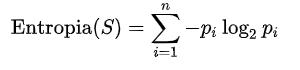
\includegraphics{capitulo2/images/formula-entropia.png}
		\caption{Fórmula para calcular la entropía.}
		\label{fig:formula-entropia}
	\end{center}
\end{figure}

\begin{figure}[!htbp]
	\hypertarget{fig:formula-ganancia}{\hspace{1pt}}
	\begin{center}
		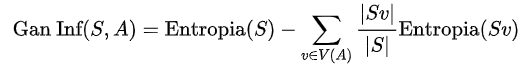
\includegraphics{capitulo2/images/formula-ganancia.png}
		\caption{Fórmula para calcular la ganancia.}
		\label{fig:formula-ganancia}
	\end{center}
\end{figure}

\newpage
\subsubsection{Ejemplo de ejecución del algoritmo ID3} \label{ejecucionID3}

Para ilustrar el funcionamiento del algoritmo ID3, utilizaremos la siguiente tabla de inducción que contiene información sobre factores que influyen al tomar la decisión de si un partido de tenis debería o no debería jugarse:

\begin{table}[!hb]
	\begin{center}
		\label{tab:tablaInduccionID3}
		\begin{tabular}{c|c|c|c|c|c}
			\textbf{Día} & \textbf{Aspecto} & \textbf{Temperatura} & \textbf{Humedad} & \textbf{Viento} & \textbf{Decisión}\\
			\hline
			1 & Soleado & Caluroso & Alta & Ligero & No\\
			2 & Soleado & Caluroso & Alta & Fuerte & No\\
			3 & Nublado & Caluroso & Alta & Ligero & Sí\\
			4 & Lluvioso & Templado & Alta & Ligero & Sí\\
			5 & Lluvioso & Fresco & Normal & Ligero & Sí\\
			6 & Lluvioso & Fresco & Normal & Fuerte & No\\
			7 & Nublado & Fresco & Normal & Fuerte & Sí\\
			8 & Soleado & Templado & Alta & Ligero & No\\
			9 & Soleado & Fresco & Normal & Ligero & Sí\\
			10 & Lluvioso & Templado & Normal & Ligero & Sí\\
			11 & Soleado & Templado & Normal & Fuerte & Sí\\
			12 & Nublado & Templado & Alta & Fuerte & Sí\\
			13 & Nublado & Caluroso & Normal & Ligero & Sí\\
			14 & Lluvioso & Templado & Alta & Fuerte & No\\
		\end{tabular}
	\end{center}
	\caption{Tabla de inducción para juegos de tenis ID3.}
\end{table}

Necesitaremos de la \refIU{fig:formula-entropia}{fórmula para calcular la entropía} y de la \refIU{fig:formula-ganancia}{fórmula para calcular la ganancia} para poder proceder con la ejecución del algoritmo.\\

\begin{UClist}
	\UCli Primeramente se calcula la entropía. La columna de \textbf{Decisión} consta de 14 instancias e incluye dos posibles valores: \textbf{sí} y \textbf{no}. Hay 9 decisiones con la etiqueta \textbf{sí} y 5 con la etiqueta \textbf{no}. Utilizando la fórmula de la entropía, se encuentra que el resultado es de \emph{0.940}.\\
	\UCli Después de los 5 factores disponibles, se busca el factor más dominante para tomar la decisión. Utilizando la fórmula de la ganancia tomando como parámetros la entropía de la columna \textbf{Decisión} y \textbf{Viento}.\\
	\UCli El atributo de viento tiene dos posibles valores: \textbf{fuerte} y \textbf{ligero}. Y al reflejar estos dos posibles valores en la fórmula, ésta se vería más o menos así: \emph{Ganancia(Decisión, Viento) = Entropía(Decisión) - [p(Decisión, Viento = Ligero)*Entropía(Decisión, Viento = Ligero)]-[p(Decisión, Viento = Fuerte)*Entropía(Decisión, Viento = Fuerte)]}.\\
	\UCli Ahora se calcula \emph{(Decisión, Viento = Ligero)} y \emph{(Decisión, Viento = Fuerte)} respectivamente.\\

	\begin{table}[!hb]
		\begin{center}
			\label{tab:tablaInduccionVientoLigero}
			\begin{tabular}{c|c|c|c|c|c}
				\textbf{Día} & \textbf{Aspecto} & \textbf{Temperatura} & \textbf{Humedad} & \textbf{Viento} & \textbf{Decisión}\\
				\hline
				1 & Soleado & Caluroso & Alta & Ligero & No\\
				3 & Nublado & Caluroso & Alta & Ligero & Sí\\
				4 & Lluvioso & Templado & Alta & Ligero & Sí\\
				5 & Lluvioso & Fresco & Normal & Ligero & Sí\\
				8 & Soleado & Templado & Alta & Ligero & No\\
				9 & Soleado & Fresco & Normal & Ligero & Sí\\
				10 & Lluvioso & Templado & Normal & Ligero & Sí\\
				13 & Nublado & Caluroso & Normal & Ligero & Sí\\
			\end{tabular}
		\end{center}
		\caption{Tabla de para el factor de decisión \emph{Viento Ligero}.}
	\end{table}

	Dentro de la tabla de viento ligero hay 8 instancias en total, de las cuales 2 tienen la decisión final \textbf{no} y 6 tienen la decisión final \textbf{sí}. Al introducir estos datos en la \refIU{fig:formula-entropia}{fórmula de la entropía}, y obtenemos una entropía de \emph{0.811}.\\

	\newpage
	\begin{table}[!hb]
		\begin{center}
			\label{tab:tablaInduccionVientoFuerte}
			\begin{tabular}{c|c|c|c|c|c}
				\textbf{Día} & \textbf{Aspecto} & \textbf{Temperatura} & \textbf{Humedad} & \textbf{Viento} & \textbf{Decisión}\\
				\hline
				2 & Soleado & Caluroso & Alta & Fuerte & No\\
				6 & Lluvioso & Fresco & Normal & Fuerte & No\\
				7 & Nublado & Fresco & Normal & Fuerte & Sí\\
				11 & Soleado & Templado & Normal & Fuerte & Sí\\
				12 & Nublado & Templado & Alta & Fuerte & Sí\\
				14 & Lluvioso & Templado & Alta & Fuerte & No\\
			\end{tabular}
		\end{center}
		\caption{Tabla de para el factor de decisión \emph{Viento Fuerte}.}
	\end{table}

	En la tabla de viento fuerte encontramos 6 instancias divididas en 2 partes iguales: 3 tienen la decisión final \textbf{sí} y 3 tienen la decisión final \textbf{no}. Al sustituir estos datos en la \refIU{fig:formula-entropia}{fórmula de la entropía}, obtenemos una entropía de \emph{1}.\\

	\UCli Ahora que tenemos esos dos valores, podemos volver a la ecuación de la ganancia. El resultado queda expresado como \emph{Ganancia(Decisión, Viento) = 0.940-[(8/14)*0.811]-[(6/14)*1] = 0.048}.\\

	\UCli En este punto se ha concluido ya el cálculo para el factor de decisión \emph{Viento}. Ahora se necesita hacer lo mismo para todas las demas colúmnas/factores.\\

	\UCli A modo de resumen:

	\begin{enumerate}
		\item Ganancia(Decisión, Aspecto) = 0.246
		\item Ganancia(Decisión, Temperatura) = 0.029
		\item Ganancia(Decisión, Humedad) = 0.151
	\end{enumerate}

	\UCli Como podemos ver, el factor de decisión \emph{Aspecto} es el que produce el valor de ganancia más alto. Por tal motivo, ese factor de decisión será el nodo raíz del árbol de decisión.\\

	\UCli Ahora debemos probar todos los valores posibles que tiene el factor de decisión \emph{Aspecto}:\\

	\UCli Aspecto Nublado\\
	\begin{table}[H]
		\begin{center}
			\label{tab:tablaInduccionAspectoNublado}
			\begin{tabular}{c|c|c|c|c|c}
				\textbf{Día} & \textbf{Aspecto} & \textbf{Temperatura} & \textbf{Humedad} & \textbf{Viento} & \textbf{Decisión}\\
				\hline
				3 & Nublado & Caluroso & Alta & Ligero & Sí\\
				7 & Nublado & Fresco & Normal & Fuerte & Sí\\
				12 & Nublado & Templado & Alta & Fuerte & Sí\\
				13 & Nublado & Caluroso & Normal & Ligero & Sí\\
			\end{tabular}
		\end{center}
		\caption{Tabla de días con aspecto \emph{nublado}.}
	\end{table}

	Podemos observar que siempre que el aspecto del día sea \textbf{nublado}, la decisión final sería \textbf{sí}.\\

	\UCli Aspecto Soleado\\
	\begin{table}[H]
		\begin{center}
			\label{tab:tablaInduccionAspectoSoleado}
			\begin{tabular}{c|c|c|c|c|c}
				\textbf{Día} & \textbf{Aspecto} & \textbf{Temperatura} & \textbf{Humedad} & \textbf{Viento} & \textbf{Decisión}\\
				\hline
				1 & Soleado & Caluroso & Alta & Ligero & No\\
				2 & Soleado & Caluroso & Alta & Fuerte & No\\
				8 & Soleado & Templado & Alta & Ligero & No\\
				9 & Soleado & Fresco & Normal & Ligero & Sí\\
				11 & Soleado & Templado & Normal & Fuerte & Sí\\
			\end{tabular}
		\end{center}
		\caption{Tabla días con aspecto \emph{soleado}.}
	\end{table}

	En esta tabla tenemos 5 instancias para el aspecto \textbf{soleado}. Hay 3 de esas instancias que tienen como decisión final \textbf{sí} y 2 que tienen \textbf{no}. Por lo que los valores de ganancia del factor de decisión \textbf{Aspecto Soleado} con respecto a todos los demás factores de decisión quedarán de la siguiente manera:\\

	\begin{enumerate}
		\item Ganancia(Aspecto = Soleado, Temperatura) = 0.570
		\item Ganancia(Aspecto = Soleado, Humedad) = 0.970
		\item Ganancia(Aspecto = Soleado, Viento) = 0.019
	\end{enumerate}

	En este punto, la humedad es el factor de decisión con mayor ganancia cuando el aspecto del día es soleado. Por lo que debemos probar todos los valores posibles para el factor de decisión \emph{humedad}.\\

	\begin{table}[H]
		\begin{center}
			\label{tab:tablaInduccionAspectoSoleadoHumedadAlta}
			\begin{tabular}{c|c|c|c|c|c}
				\textbf{Día} & \textbf{Aspecto} & \textbf{Temperatura} & \textbf{Humedad} & \textbf{Viento} & \textbf{Decisión}\\
				\hline
				1 & Soleado & Caluroso & Alta & Ligero & No\\
				2 & Soleado & Caluroso & Alta & Fuerte & No\\
				8 & Soleado & Templado & Alta & Ligero & No\\
			\end{tabular}
		\end{center}
		\caption{Tabla días con aspecto \emph{soleado} y humedad \emph{alta}.}
	\end{table}

	La decisión siempre será \textbf{no} cuando la humedad sea \textbf{alta}.\\

	\begin{table}[H]
		\begin{center}
			\label{tab:tablaInduccionAspectoSoleadoHumedadNormal}
			\begin{tabular}{c|c|c|c|c|c}
				\textbf{Día} & \textbf{Aspecto} & \textbf{Temperatura} & \textbf{Humedad} & \textbf{Viento} & \textbf{Decisión}\\
				\hline
				9 & Soleado & Fresco & Normal & Ligero & Sí\\
				11 & Soleado & Templado & Normal & Fuerte & Sí\\
			\end{tabular}
		\end{center}
		\caption{Tabla días con aspecto \emph{soleado} y humedad \emph{normal}.}
	\end{table}

	Por otro lado, la decisión siempre será \textbf{sí} cuando la humedad es \textbf{normal}.\\

	De lo anterior concluimos que deberemos verificar la humedad y decidir si el aspecto del día es \textbf{soleado}.\\

	\UCli Aspecto Lluvioso\\
	\begin{table}[H]
		\begin{center}
			\label{tab:tablaInduccionAspectoLluvioso}
			\begin{tabular}{c|c|c|c|c|c}
				\textbf{Día} & \textbf{Aspecto} & \textbf{Temperatura} & \textbf{Humedad} & \textbf{Viento} & \textbf{Decisión}\\
				\hline
				4 & Lluvioso & Templado & Alta & Ligero & Sí\\
				5 & Lluvioso & Fresco & Normal & Ligero & Sí\\
				6 & Lluvioso & Fresco & Normal & Fuerte & No\\
				10 & Lluvioso & Templado & Normal & Ligero & Sí\\
				14 & Lluvioso & Templado & Alta & Fuerte & No\\
			\end{tabular}
		\end{center}
		\caption{Tabla de días con aspecto \emph{lluvioso}.}
	\end{table}

	Al evaluar los valores de ganancia de los días con aspecto \textbf{lluvioso} con respecto a los demás factores de decisión, se encuentra que el factor que genera una mayor ganancia es el viento. Por lo cual se tienen que checar todos los posibles valores de ese factor de decisión.\\

	\begin{table}[H]
		\begin{center}
			\label{tab:tablaInduccionAspectoLluviosoVientoLigero}
			\begin{tabular}{c|c|c|c|c|c}
				\textbf{Día} & \textbf{Aspecto} & \textbf{Temperatura} & \textbf{Humedad} & \textbf{Viento} & \textbf{Decisión}\\
				\hline
				4 & Lluvioso & Templado & Alta & Ligero & Sí\\
				5 & Lluvioso & Fresco & Normal & Ligero & Sí\\
				10 & Lluvioso & Templado & Normal & Ligero & Sí\\
			\end{tabular}
		\end{center}
		\caption{Tabla de días con aspecto \emph{lluvioso} y con viento \emph{ligero}.}
	\end{table}

	De la tabla de aspecto \textbf{lluvioso} y viento \textbf{ligero} podemos deducir que siempre que existan estas dos condiciones al mismo tiempo, la decisión final será \textbf{sí}.\\

	\begin{table}[H]
		\begin{center}
			\label{tab:tablaInduccionAspectoLluvioso}
			\begin{tabular}{c|c|c|c|c|c}
				\textbf{Día} & \textbf{Aspecto} & \textbf{Temperatura} & \textbf{Humedad} & \textbf{Viento} & \textbf{Decisión}\\
				\hline
				6 & Lluvioso & Fresco & Normal & Fuerte & No\\
				14 & Lluvioso & Templado & Alta & Fuerte & No\\
			\end{tabular}
		\end{center}
		\caption{Tabla de días con aspecto \emph{lluvioso}.}
	\end{table}
	\newpage
	De la tabla de aspecto \textbf{lluvioso} y viento \textbf{fuerte} podemos deducir que siempre que existan estas dos condiciones al mismo tiempo, la decisión final será \textbf{no}.\\

	\UCli Finalmente la construcción de este árbol de decisión es la siguiente:

	\begin{figure}[H]
		\hypertarget{fig:arbol-decision-final}{\hspace{1pt}}
		\begin{center}
			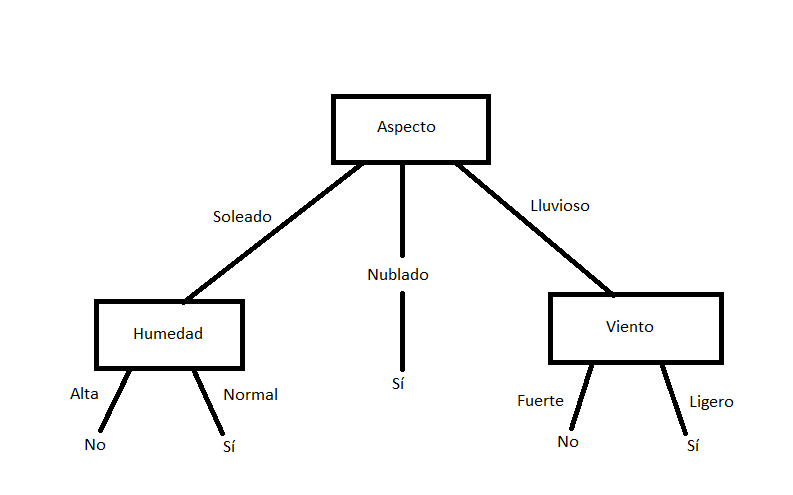
\includegraphics{capitulo2/images/arbol-decision-final.png}
			\caption{Árbol de decisión resultante.}
			\label{fig:arbol-decision-final}
		\end{center}
	\end{figure}
\end{UClist}
\subsection{C4.5} \label{c4.5}
El algoritmo C4.5 es la evolución del algoritmo ID3. Éste genera un árbol de decisión a partir de un conjunto de datos de entrada de manera recursiva, al igual que su precursor\cite{c4.5}. Sin embargo, aunque ID3 y C4.5 son algoritmos muy semejantes, existen ciertas diferencias:\\

\begin{UClist}
	\UCli C4.5 permite trabajar con valores continuos, mientras que ID3 solamente trabaja con valores discretos.\\
	\UCli Los árboles de C4.5 son más compactos, y esto se debe a que cada nodo hoja engloba un conjunto de clases y no una sola clase particular.\\
	\UCli C4.5 es más eficiente computacionalmente hablando.\\
	\UCli C4.5 utiliza un nuevo parámetro llamado \textbf{Gain Ratio}, en lugar de la ganancia simple. Y este a su vez requiere de la ganancia y de otro parámetro nuevo llamado \textbf{SplitInfo} cuyas fórmulas se enuncian a continuación\cite{c4.5}:
	
	\begin{figure}[H]
		\hypertarget{fig:formula-gainratio}{\hspace{1pt}}
		\begin{center}
			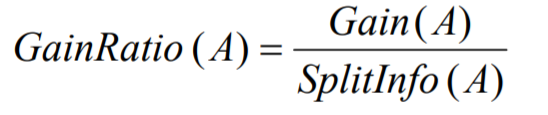
\includegraphics[width=0.5\textwidth]{capitulo2/images/formula-gainratio.png}
			\caption{Fórmula para obtener el Gain Ratio}
			\label{fig:formula-gainratio}
		\end{center}
	\end{figure}

	\begin{figure}[H]
		\hypertarget{fig:formula-splitinfo}{\hspace{1pt}}
		\begin{center}
			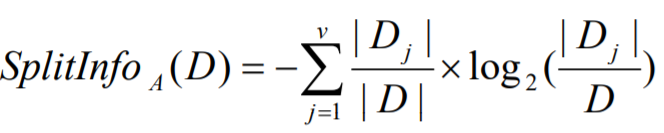
\includegraphics[width=0.5\textwidth]{capitulo2/images/formula-splitinfo.png}
			\caption{Fórmula para obtener SplitInfo}
			\label{fig:formula-splitinfo}
		\end{center}
	\end{figure}

\end{UClist}

\subsubsection{Ejemplo de ejecución del algoritmo C4.5}
Para mostrar la forma en la que se ejecuta el algoritmo C4.5 y los pasos que se deben llevar a cabo, se utilizará la siguiente tabla de inducción:

\begin{table}[H]
	\begin{center}
		\label{tab:tablaInduccionC4.5}
		\begin{tabular}{c|c|c|c|c|c}
			\textbf{Día} & \textbf{Aspecto} & \textbf{Temperatura} & \textbf{Humedad} & \textbf{Viento} & \textbf{Decisión}\\
			\hline
			1 & Soleado & 85 & 85 & Ligero & No\\
			2 & Soleado & 80 & 90 & Fuerte & No\\
			3 & Nublado & 83 & 78 & Ligero & Sí\\
			4 & Lluvioso & 70 & 96 & Ligero & Sí\\
			5 & Lluvioso & 68 & 80 & Ligero & Sí\\
			6 & Lluvioso & 65 & 70 & Fuerte & No\\
			7 & Nublado & 64 & 65 & Fuerte & Sí\\
			8 & Soleado & 72 & 95 & Ligero & No\\
			9 & Soleado & 69 & 70 & Ligero & Sí\\
			10 & Lluvioso & 75 & 80 & Ligero & Sí\\
			11 & Soleado & 75 & 70 & Fuerte & Sí\\
			12 & Nublado & 72 & 90 & Fuerte & Sí\\
			13 & Nublado & 81 & 75 & Ligero & Sí\\
			14 & Lluvioso & 80 & 80 & Fuerte & No\\
		\end{tabular}
	\end{center}
	\caption{Tabla de inducción para juegos de tenis C4.5.}
\end{table}

\begin{UClist}
	\UCli Al igual que con el ejemplo \nameref{ejecucionID3}, lo primero que se hace es calcular la entropía general. Hay 15 instancias de las cuales 9 tienen una decisión final de \textbf{sí} y 5 tienen \textbf{no}. Al sustituir los valores correspondientes en la \refIU{fig:formula-entropia}{fórmula para calcular la entropía} el resultado que obtenemos es \emph{0.940}.\\

	\UCli En C4.5 se utilizan \textbf{Gain Ratios} (radios de ganancia), mientras que en ID3 se utilizan ganancias.\\

	\UCli Empezaremos por analizar el atributo de \textbf{Viento}.\\

	Se tienen 8 instancias de \emph{viento ligero}, dos de ellas concluyen en un \textbf{no}, y las otras 6 concluyen en \textbf{sí} por lo que:\\

	\begin{enumerate}
		\item Entropía(Decisión, Viento = Ligero) = 0.811\\
		\item Entropía(Decisión, Viento = Fuerte) = 1\\
		\item Ganancia(Decisión, Viento) = 0.049\\
	\end{enumerate}

	Existen 6 instancias de viento fuerte por lo que:

	\begin{enumerate}
		\item SplitInfo(Decisión, Viento) = 0.985\\
		\item GainRatio(Decisión, Viento) = Gain(Decisión, Viento) / SplitInfo(Decision, Viento) = 0.049\\
	\end{enumerate}

	\UCli Continuamos analizando ahora el atributo \textbf{Aspecto}.\\

	Se tienen 5 instancias para el aspecto \emph{soleado}, de las cuales 3 concluyen en \textbf{no} y las otras 2 concluyen en \textbf{sí}. Calculando sus valores de entropías, ganancia, SplitInfo y GainRatio:\\

	\begin{enumerate}
		\item Entropía(Decisión, Aspecto = Soleado) = 0.970\\
		\item Entropía(Decisión, Aspecto = Nublado) = 0\\
		\item Entropía(Decisión, Aspecto = Lluvioso) = 0.970\\
		\item Ganancia(Decisión, Aspecto) = 0.246\\
		Hay 5 instancias para \emph{soleado}, 4 instancias para \emph{nublado} y 5 para \emph{lluvioso}, por lo que:\\
		\item SplitInfo(Decisión, Aspecto) = 1.577\\
		\item GainRatio(Decisión, Aspecto) = 0.155\\
	\end{enumerate}

	\UCli Procedemos a analizar el atributo de humedad. Cuyo caso es diferente al de los demás atributos, ya que este es un atributo continuo. Necesitamos convertir valoress continuos a valores nominales (como todos los demás atributos). C4.5 propone hacer una división binaria a partir de algún valor que podamos tomar como umbral. El umbral debe ser el valor que mayor ganancia ofrezca para ese atributo. Para esto, primero se deben ordenar las instancias de humedad de menor a mayor.\\

	\begin{table}[H]
		\begin{center}
			\label{tab:tablaInduccionC4.5Humedad}
			\begin{tabular}{c|c|c}
				\textbf{Día} & \textbf{Humedad} & \textbf{Decisión}\\
				\hline
				7 & 65 & Sí\\
				6 & 70 & No\\
				9 & 70 & Sí\\
				11 & 70 & Sí\\
				13 & 75 & Sí\\
				3 & 78 & Sí\\
				5 & 80 & Sí\\
				10 & 80 & Sí\\
				14 & 80 & No\\
				1 & 85 & No\\
				2 & 90 & No\\
				12 & 90 & Sí\\
				8 & 95 & No\\
				4 & 96 & Sí\\
			\end{tabular}
		\end{center}
		\caption{Tabla de l atributo \emph{humedad} ordenada de menor a mayor.}
	\end{table}

	Ahora debemos recorrer todos los valores de humedad y separar el conjunto de datos en dos partes. Se calcularán la \textbf{Ganancia} y el \textbf{GainRatio} y el valor que maximice la ganancia será el umbral.\\

	\begin{enumerate}
		\item Se propone 65 como umbral.
		\begin{enumerate}
			\item Entropía(Decisión, Humedad <= 65) = 0
			\item Entropía(Decisión, Humedad > 65) = 0.961
			\item Ganancia(Decisión, Humedad <> 65) = 0.048
			\item SplitInfo(Decisión, Humedad <> 65) = 0.371
			\item GainRatio(Decisión, Humedad <> 65) = 0.126\\
		\end{enumerate}
		\item Se propone 70 como umbral.
		\begin{enumerate}
			\item Entropía(Decisión, Humedad <= 70) = 0.811
			\item Entropía(Decisión, Humedad > 70) = 0.970
			\item Ganancia(Decisión, Humedad <> 70) = 0.014
			\item SplitInfo(Decisión, Humedad <> 70) = 0.863
			\item GainRatio(Decisión, Humedad <> 70) = 0.016\\
		\end{enumerate}
		\item Se propone 75 como umbral.
		\begin{enumerate}
			\item Entropía(Decisión, Humedad <= 75) = 0.721
			\item Entropía(Decisión, Humedad > 75) = 0.991
			\item Ganancia(Decisión, Humedad <> 75) = 0.045
			\item SplitInfo(Decisión, Humedad <> 75) = 0.940
			\item GainRatio(Decisión, Humedad <> 75) = 0.047\\
		\end{enumerate}
		\item Se continúa haciendo lo mismo para cada valor nuevo de humedad que se vaya encontrando en la tabla. Resumiendo:
		\item Ganancia(Decisión, Humedad <> 78) = 0.090
		\item Ganancia(Decisión, Humedad <> 80) = 0.107
		\item Ganancia(Decisión, Humedad <> 85) = 0.027
		\item Ganancia(Decisión, Humedad <> 90) = 0.016
	\end{enumerate}

	\UCli Como podemos ver, el valor que maximiza la ganancia es el de 80. Lo que significa que ahora se debe comparar los otros valores nominales con el valor 80 del atributo \emph{humedad} para crear una rama en nuestro árbol. De esta forma podemos resumir los resultados en la siguiente tabla:\\

	\begin{table}[H]
		\label{tab:tablaComparacionHumedadAtributos}
		\begin{center}
			\begin{tabular}{c|c|c}
				\textbf{Atributo} & \textbf{Ganancia} & \textbf{GainRatio}\\
				\hline
				Viento & 0.049 & 0.049\\
				Aspecto & 0.246 & 0.155\\
				Humedad <> 80 & 0.101 & 0.107\\
			\end{tabular}
			\caption{Comparación de las ganancias entre atributos.}
		\end{center}
	\end{table} 

	\UCli Al igual que en el ejemplo del algoritmo ID3, el atributo \textbf{aspecto} es el nodo raíz del árbol de decisión, por lo que ahora se deben analizar todos los posibles valores que puede adquirir dicho atributo.\\

	\UCli Aspecto Soleado.\\

	\begin{table}[H]
		\begin{center}
			\label{tab:tablaSoleadoC4.5}
			\begin{tabular}{c|c|c|c|c|c}
				\textbf{Día} & \textbf{Aspecto} & \textbf{Temperatura} & \textbf{Humedad} & \textbf{Viento} & \textbf{Decisión}\\
				\hline
				1 & Soleado & 85 & 85 & Ligero & No\\
				2 & Soleado & 80 & 90 & Fuerte & No\\
				8 & Soleado & 72 & 95 & Ligero & No\\
				9 & Soleado & 69 & 70 & Ligero & Sí\\
				11 & Soleado & 75 & 70 & Fuerte & Sí\\
			\end{tabular}
		\end{center}
		\caption{Tabla de inducción para el atributo \emph{Aspecto} con el valor \emph{Soleado}.}
	\end{table}

	Ya hemos dividido la humedad a partir de su punto de umbral que es 80. Podemos observar en la siguiente tabla que la decisión final será \textbf{no}, si la humedad es mayor a 80 y el aspecto del día es soleado. La decisión final será \textbf{sí}, si la humedad es menor o igual a 80 para un día soleado.\\

	\begin{table}[H]
		\begin{center}
			\label{tab:tablaNubladoC4.5}
			\begin{tabular}{c|c|c|c|c|c}
				\textbf{Día} & \textbf{Aspecto} & \textbf{Temperatura} & \textbf{Humedad} & \textbf{Viento} & \textbf{Decisión}\\
				\hline
				3 & Nublado & 83 & 78 & Ligero & Sí\\
				7 & Nublado & 64 & 65 & Fuerte & Sí\\
				12 & Nublado & 72 & 90 & Fuerte & Sí\\
				13 & Nublado & 81 & 75 & Ligero & Sí\\
			\end{tabular}
		\end{center}
		\caption{Tabla de inducción para el atributo \emph{Aspecto} con el valor \emph{Nublado}.}
	\end{table}

	Cuando el aspecto del día es \textbf{nublado}, no importa ninguna otra condición; ni temperatura, ni humedad. La decisión final siempre será \textbf{sí}.\\

	\begin{table}[H]
		\begin{center}
			\label{tab:tablaLluviosoC4.5}
			\begin{tabular}{c|c|c|c|c|c}
				\textbf{Día} & \textbf{Aspecto} & \textbf{Temperatura} & \textbf{Humedad} & \textbf{Viento} & \textbf{Decisión}\\
				\hline
				4 & Lluvioso & 70 & 96 & Ligero & Sí\\
				5 & Lluvioso & 68 & 80 & Ligero & Sí\\
				6 & Lluvioso & 65 & 70 & Fuerte & No\\
				10 & Lluvioso & 75 & 80 & Ligero & Sí\\
				14 & Lluvioso & 80 & 80 & Fuerte & No\\
			\end{tabular}
		\end{center}
		\caption{Tabla de inducción para el atributo \emph{Aspecto} con el valor \emph{Lluvioso}.}
	\end{table}

	Cuando el aspecto es \textbf{lluvioso}, la decisión será \textbf{sí} cuando el viento es ligero, y será \textbf{no} cuando sea fuerte.\\

	\UCli De todo lo anterior se concluye un árbol de decisión con la siguiente estructura:\\

	\begin{figure}[H]
		\hypertarget{fig:arbol-final-c45}{\hspace{1pt}}
		\begin{center}
			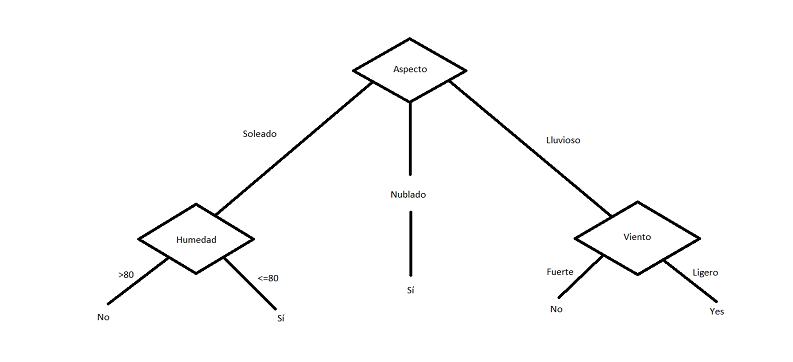
\includegraphics{capitulo2/images/arbol-final-c45.png}
			\caption{Arbol de decisión construido con C4.5.}
			\label{fig:arbol-final-c45}
		\end{center}
	\end{figure}

\end{UClist}

\newpage
\subsection{Algoritmo KNN (K-Nearest Neighbor)}
El algoritmo KNN es un algoritmo de aprendizaje no supervisado en el que se busca clasificar un punto en una categoría con la ayuda de un conjunto de entrenamiento \cite{KNN}.\\

Los pasos que sigue el algoritmo KNN se enumeran a continuación:\\

\begin{enumerate}
	\item Se calcula la similitud entre puntos basaándose en una función de distancia.\\
	\item Se encuentran los \emph{K} vecinos más cercanos.\\
\end{enumerate}

\subsubsection{Ejemplo de ejecución del algoritmo KNN}
Con base en la siguiente información que relaciona el peso, la altura y la talla de playera de personas, se hará la ejecución del algoritmo KNN.\\

	\begin{table}[H]
		\begin{center}
			\label{tab:tablaKNN}
			\begin{tabular}{c|c|c}
				\textbf{Altura (cm)} & \textbf{Peso (kg)} & \textbf{Talla}\\
				\hline
				158 & 58 & M\\
				158 & 59 & M\\
				158 & 63 & M\\
				160 & 59 & M\\
				160 & 60 & M\\
				163 & 60 & M\\
				163 & 61 & M\\
				160 & 64 & L\\
				163 & 64 & L\\
				165 & 61 & L\\
				165 & 62 & L\\
				165 & 65 & L\\
				168 & 62 & L\\
				168 & 63 & L\\
				168 & 66 & L\\
				170 & 63 & L\\
				170 & 64 & L\\
				170 & 68 & L\\
			\end{tabular}
		\end{center}
		\caption{Conjunto de entrenamiento para el algoritmo KNN.}
	\end{table}

\begin{UClist}
	\textbf{Nuevo dato: Altura = 161 cm, Peso = 61 kg}

	\UCli Se calcula la distancia Euclidiana entre el dato de entrada y cada uno de los datos del conjunto de entrenamiento, utilizando la siguiente fórmula.\\

	\begin{figure}[H]
		\begin{center}
			\hypertarget{fig:distanciaEuclidiana}{\hspace{1pt}}
			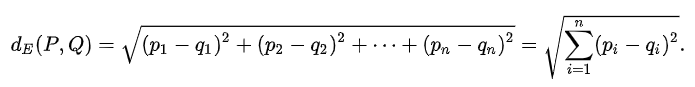
\includegraphics{capitulo2/images/distanciaEuclidiana.png}
			\caption{Fórmula para calcular la distancia Euclidiana.}
			\label{fig:distanciaEuclidiana}
		\end{center}
	\end{figure}

	Obtenemos lo siguiente:\\

	\begin{table}[H]
		\begin{center}
			\label{tab:tablaKNNDistancias}
			\begin{tabular}{c|c|c|c}
				\textbf{Altura (cm)} & \textbf{Peso (kg)} & \textbf{Talla} & \textbf{Distancia}\\
				\hline
				158 & 58 & M & 4.2\\
				158 & 59 & M & 3.6\\
				158 & 63 & M & 3.6\\
				160 & 59 & M & 2.2\\
				160 & 60 & M & 1.4\\
				163 & 60 & M & 2.2\\
				163 & 61 & M & 2.0\\
				160 & 64 & L & 3.2\\
				163 & 64 & L & 3.6\\
				165 & 61 & L & 4.0\\
				165 & 62 & L & 4.1\\
				165 & 65 & L & 5.7\\
				168 & 62 & L & 7.1\\
				168 & 63 & L & 7.3\\
				168 & 66 & L & 8.6\\
				170 & 63 & L & 9.2\\
				170 & 64 & L & 9.5\\
				170 & 68 & L & 11.4\\
			\end{tabular}
		\end{center}
		\caption{Tabla del conjunto de entrenamiento con la columna \textbf{Distancia} ya calculada.}
	\end{table}

	\UCli Se toma la distancia más pequeña para determinar al vecino más cercano de entre todas las distancias Euclidianas calculadas previamente. Esta distancia es \textbf{1.4}.\\

	\UCli Se define \emph{K} como el número de vecinos más cercanos que queramos conocer. Para este caso definiremos \emph{K} igual a 5. Por lo que se tomarán los 5 valores más pequeños.\\

	\begin{table}[H]
		\begin{center}
			\label{tab:tablaKNNDistanciasMinimas}
			\begin{tabular}{c|c|c|c}
				\textbf{Altura (cm)} & \textbf{Peso (kg)} & \textbf{Talla} & \textbf{Distancia}\\
				\hline
				160 & 60 & M & 1.4\\
				163 & 61 & M & 2.0\\
				163 & 60 & M & 2.2\\
				160 & 59 & M & 2.2\\
				160 & 64 & L & 3.2\\
			\end{tabular}
		\end{center}
		\caption{Instancias de la tabla con menor distancia al nuevo dato.}
	\end{table}

\end{UClist}

\subsection{Algoritmo K-Means}
El algoritmo K-Means es un algoritmo de agrupamiento que utiliza aprendizaje no supervisado, el cual es utilizado cuando se tienen datos no etiquetados, es decir sin categorías o grupos definidos. El objetivo de este algoritmo es encontrar grupos en los datos, con el número de grupos se representa la variable \emph{K}\cite{KMeans}. El algoritmo arrojará como resultado final lo siguiente:\\

\begin{enumerate}
	\item Los centroides de los \emph{K} grupos.\\
	\item Etiquetas para los datos de entrenamiento. Cada dato es asignado a un solo grupo.\\
\end{enumerate}

\subsubsection{Ejemplo de ejecución del algoritmo K-Means}
Para ilustrar el funcionamiento del algoritmo K-means, se utilizará el siguiente conjunto de entrenamiento correspondiente a la puntuación de 7 individuos en 2 pruebas:

\begin{table}[H]
	\begin{center}
		\label{tab:conjuntoKMeans}
		\begin{tabular}{c|c|c}
			\textbf{Individuo} & \textbf{Prueba 1} & \textbf{Prueba 2}\\
			\hline
			1 & 1.0 & 1.0\\
			2 & 1.5 & 2.0\\
			3 & 3.0 & 4.0\\
			4 & 5.0 & 7.0\\
			5 & 3.5 & 5.0\\
			6 & 4.5 & 5.0\\
			7 & 3.5 & 4.5\\
		\end{tabular}
	\end{center}
	\caption{Conjunto de entrenamiento para el algoritmo K-Means.}
\end{table}

\begin{UClist}
	\UCli El conjunto de datos se agrupa en dos grupos distintos. Para esto, se toman los valores de la \emph{Prueba 1} y \emph{Prueba 2} de los individuos que tengan estos valores más lejanos, es decir:\\

	\begin{table}[H]
		\begin{center}
			\label{tab:gruposInicialesKMeans}
			\begin{tabular}{c|c|c}
				\textbf{Grupo} & \textbf{Individuo} & \textbf{Vector (Centroide)}\\
				\hline
				Grupo 1 & 1 & (1.0, 1.0)\\
				Grupo 2 & 4 & (5.0, 7.0)\\
			\end{tabular}
		\end{center}
		\caption{Partición inicial.}
	\end{table}

	\UCli Los individuos restantes ahora son examinados secuencialmente y son ubicados en el grupo al que son más cercanos en términos de distancia Euclidiana. El vector es recalculado cada que un nuevo miembro es agregado.

	\begin{table}[H]
		\begin{center}
			\label{tab:gruposIndividuosCompletosGrupo1}
			\begin{tabular}{c|c|c}
				\textbf{Iteración} & \textbf{Individuo} & \textbf{Vector (Centroide)}\\
				\hline
				1 & 1 & (1.0, 1.0)\\
				2 & 1, 2 & (1.2, 1.5)\\
				3 & 1, 2, 3 & (1.8, 2.3)\\
				4 & 1, 2, 3 & (1.8, 2.3)\\
				5 & 1, 2, 3 & (1.8, 2.3)\\
				6 & 1, 2, 3 & (1.8, 2.3)\\
			\end{tabular}
		\end{center}
		\caption{Tabla de individuos agregados secuencialmente al \textbf{Grupo 1}.}
	\end{table}

	\begin{table}[H]
		\begin{center}
			\label{tab:gruposIndividuosCompletosGrupo2}
			\begin{tabular}{c|c|c}
				\textbf{Iteración} & \textbf{Individuo} & \textbf{Vector (Centroide)}\\
				\hline
				1 & 4 & (5.0, 7.0)\\
				2 & 4 & (5.0, 7.0)\\
				3 & 4 & (5.0, 7.0)\\
				4 & 4, 5 & (4.2, 6.0)\\
				5 & 4, 5, 6 & (4.3, 5.7)\\
				6 & 4, 5, 6, 7 & (4.1, 5.4)\\
			\end{tabular}
		\end{center}
		\caption{Tabla de individuos agregados secuencialmente al \textbf{Grupo 2}.}
	\end{table}

	\UCli Ahora la partición inicial ha cambiado, y los dos grupos tienen las siguientes características:

	\begin{table}[H]
		\begin{center}
			\label{tab:gruposModificadosKMeans}
			\begin{tabular}{c|c|c}
				\textbf{Grupo} & \textbf{Individuo} & \textbf{Vector (Centroide)}\\
				\hline
				Grupo 1 & 1, 2, 3 & (1.8, 2.3)\\
				Grupo 2 & 4, 5, 6, 7 & (4.1, 5.4)\\
			\end{tabular}
		\end{center}
		\caption{Partición inicial modificada.}
	\end{table}

	\UCli Sin embargo, no podemos asegurarnos de que esas son las clasificaciones correctas para cada dato. Así que comparamos la distancia de cada individuo a su propio grupo y al grupo opuesto:

	\begin{table}[H]
		\begin{center}
			\label{tab:distanciasACadaGrupo}
			\begin{tabular}{c|c|c}
				\textbf{Individuo} & \textbf{Distancia al Grupo 1} & \textbf{Distancia al Grupo 2}\\
				\hline
				1 & 1.5 & 5.4\\
				2 & 0.4 & 4.3\\
				3 & 2.1 & 1.8\\
				4 & 5.7 & 1.8\\
				5 & 3.2 & 0.7\\
				6 & 3.8 & 0.6\\
				7 & 2.8 & 1.1\\
			\end{tabular}
		\end{center}
		\caption{Cálculo de distancia de cada dato a su grupo y al opuesto.}
	\end{table}

	\UCli Solamente el individuo 3 está más cerca al centroide del grupo opuesto (Grupo 2) que de su propio grupo (Grupo 1). Por lo que el individuo 3 se reubica en el Grupo 2. Resultando la siguiente partición:\\

	\begin{table}[H]
		\begin{center}
			\label{tab:particionFinal}
			\begin{tabular}{c|c|c}
				\textbf{Grupo} & \textbf{Individuo} & \textbf{Vector (Centroide)}\\
				\hline
				Grupo 1 & 1, 2 & (1.8, 1.5)\\
				Grupo 2 & 3, 4, 5, 6, 7 & (3.9, 5.1)\\
			\end{tabular}
		\end{center}
		\caption{Partición final.}
	\end{table}

	\UCli Las iteraciones continuarían hasta que ya no haya más reubicaciones.\\

	\UCli Es probable que el algoritmo no encuentre una solución final.

\end{UClist}

\subsection{MapReduce}
MapReduce es un paradigma de programación que permite escalabilidad masiva a través de cientos o miles de servidores en un clúster Hadoop. \emph{MapReduce} se refiere a dos tareas distintas y separadas. La primera, \emph{Map}, consiste en realizar mapeos. Ésta convierte un conjunto de datos en otro conjunto de datos diferente en el que los elementos individuales son separados en tuplas. La segunda, \emph{Reduce}, toma los datos que arroja de \emph{Map}, y combina esas tuplas en un conjunto más pequeño de tuplas. MapReduce es el corazón de Hadoop.\cite{mapReduce}\\

\subsection{Hadoop} \label{sect:hadoop}
Es un framework de software que soporta aplicaciones distribuidas bajo una licencia libre. Permite a las aplicaciones trabajar con miles de nodos y petabytes de datos. Hadoop se inspiró en los documentos Google para MapReduce y Google File System (GFS). Hadoop utiliza su propio sistema de archivos HDFS, que divide archivos grandes y los distribuye en diferentes nodos para su procesamiento.\cite{hadoop}\\

\subsubsection{Características principales de Hadoop}

\begin{UClist}
	\UCli \textbf{Procesamiento distribuido:} Hadoop distribuye los datos en los diferentes nodos que formen parte de la arquitectura de clúster que estén haciendo uso de él. Pretende paralelizar tareas de procesamiento de datos\cite{hadoop}.\\
	\UCli \textbf{Eficiencia:} Mediante la paralelización, se consigue una ganancia considerable en el tiempo de procesamiento de información.\cite{hadoop}\\
	\UCli \textbf{Económico:} Propicia un ambiente fácilmente escalable en el que resulta sencillo añadir nodos de manera horizontal conforme se vaya requiriendo.\cite{hadoop}\\
	\UCli \textbf{Código abierto:} Es un proyecto de los llamados \textbf{open source}.\cite{hadoop}\\
	\UCli \textbf{Tolerancia a fallos:} Utiliza replicación de datos haciendo uso de \textbf{HDFS (Hadoop Distributed File System)}. Si un nodo falla o cae, hay nodos de respaldo que permiten mantener el ambiente en funcionamiento.\cite{hadoop}\\
\end{UClist}

\newpage
\subsubsection{Arquitectura de Hadoop}
\begin{figure}[H]
	\begin{center}
		\hypertarget{fig:hadoopComponentes}{\hspace{1pt}}
		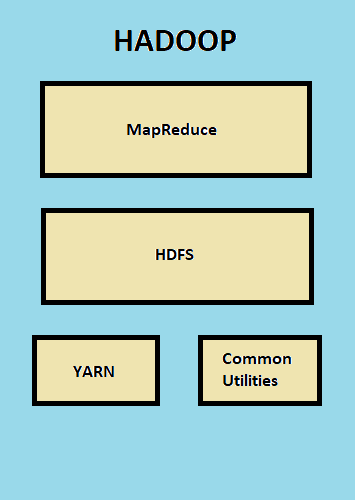
\includegraphics{capitulo2/images/hadoopComponentes.png}
		\caption{Arquitectura básica de Hadoop.}
		\label{fig:hadoopComponentes}
	\end{center}
\end{figure}

\begin{UClist}
	\UCli \textbf{MapReduce:} Es el módulo que permite ejecutar cómputo distribuido. Pretende la paralelización de procesos.\\
	\UCli \textbf{HDFS (Hadoop Distributed File System:)} Es el sistema de archivos distribuido que utiliza Hadoop. Éste parte los datos en fragmentos y los almacena en los nodos que conforman el clúster donde Hadoop esté ejecutándose.\\
	\UCli \textbf{YARN:} Es el gestor de recursos de Hadoop.\\
	\UCli \textbf{Common Utilities:} Librerías y código necesario para ejecutar Hadoop.\\
\end{UClist}

\newpage
\subsubsection{Arquitectura de un clúster Hadoop}
Habitualmente, un clúster Hadoop tiene la estructura \textbf{\emph{maestro - esclavo}}. Lo que significa que hay un nodo \textbf{maestro} que estará coordinando la ejecución de tareas y las asignará a los nodos \textbf{esclavos}.\\

\begin{figure}[H]
	\begin{center}
		\hypertarget{fig:arquitecturaMaestroEsclavo}{\hspace{1pt}}
		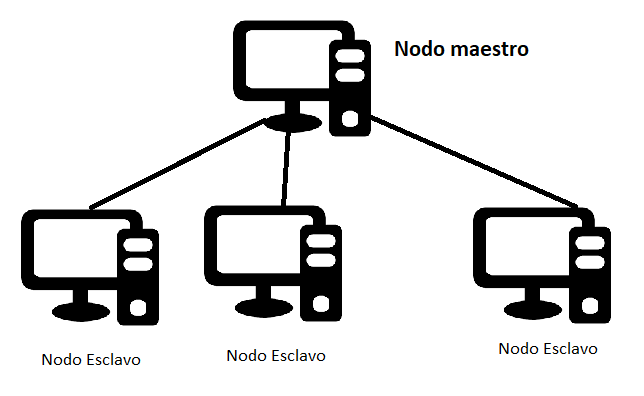
\includegraphics{capitulo2/images/arquitecturaMaestroEsclavo.png}
		\caption{Arquitectura de maestros y esclavos.}
		\label{fig:arquitecturaMaestroEsclavo}
	\end{center}
\end{figure}

\subsubsection{Distribuciones Comerciales de Hadoop}
Existen varias opciones actualmente en el mercado para hacer uso de las capacidades de Hadoop, entre las cuales destacan 3 principalmente\cite{distH}:\\

\begin{UClist}
	\UCli \textbf{Cloudera:} Fue la primera de todas las distribuciones comerciales de Hadoop. Cuenta con una herramienta llamada Cloudera Manager que permite gestionar el clúster.\\
	\UCli \textbf{Hortonworks:} Es la distribución de Hadoop más nueva. Permite instalar el clúster mediante un cliente de virtualización.\\
	\UCli \textbf{Microsoft Azure:} Es una distribución desarrollada por Microsoft que permite tener las máquinas del clúster en la nube.\\
\end{UClist}

\subsection{Apache Spark}
Es un motor de análisis de datos unificado para Big Data y Machine Learning. Que se basa en Hadoop Map Reduce. Es una herramienta de código abierto que permite \textbf{dividir y ejecutar tareas de manera paralela}. Esta cualidad de Spark de poder paralelizar el trabajo se debe a que éste software en la gran mayoría de los casos es ejecutado en sistemas con arquitectura de clúster.\cite{spark} \\
\newpage
\subsubsection{Características principales de Spark}
\begin{UClist}
	\UCli Integrado con Apache Hadoop.\\
	\UCli Ofrece un desempeño veloz.\\
	\UCli El almacenamiento de datos se administra en memoria. Se reducen mucho los tiempos de ejecución ya que hay muchas menos operaciones de lectura y escritura en disco.\\
	\UCli Puede ejecutar algoritmos escritos en Java, Scala, Python y R.\\
	\UCli Permite procesamiento en tiempo real.\\
\end{UClist}

\subsubsection{Ventajas de usar Apache Spark}
Utilizar Spark para el procesamiento de volúmenes de información de gran tamaño ofrece varios beneficios.\cite{spark} Los principales beneficios son los siguientes:\\

\begin{UClist}
	\UCli \textbf{Velocidad:} Gran velocidad en el procesamiento de información. Esto se debe a lo ya mencionado anteriormente sobre la gestion de datos desde memoria.\\
	\UCli \textbf{Potencia:} Spark nos permite aprovechar el hardware de los equipos que lo estén utilizando.\\

	\UCli \textbf{Fácil uso:} A diferencia de Hadoop, que requería de un amplio conocimiento de MapReduce y de Java, Spark permite usar lenguajes de más alto nivel como Python y Scala además de Java.\\

	\UCli \textbf{Integración SQL:} Como resultado de contener el módulo Spark SQL, es posible realizar consultas en conjuntos de datos semi-estructurados utilizando lenguaje SQL.\\

	\UCli \textbf{Constante mejora del propio sistema:} Al ser un proyecto de código abierto, cada vez hay más personas que contribuyen a la mejora y ampliación de los alcances de Spark.\\

	\UCli \textbf{Escalabilidad:} Spark permite que incrementar el tamaño del clúster conforme se vaya necesitando.\\
\end{UClist}
\newpage
\subsubsection{Componentes de Apache Spark}
Podría decirse que Spark es un conjunto de módulos que nos permiten generar conocimiento usando diferentes técnicas y tecnologías\cite{spark}.\\

El diagrama mostrado a continuación ilustra los principales módulos o \textbf{componentes} que conforman Apache Spark.\\

\begin{figure}[H]
	\hypertarget{fig:sparkComponentes}{\hspace{1pt}}
	\begin{center}
		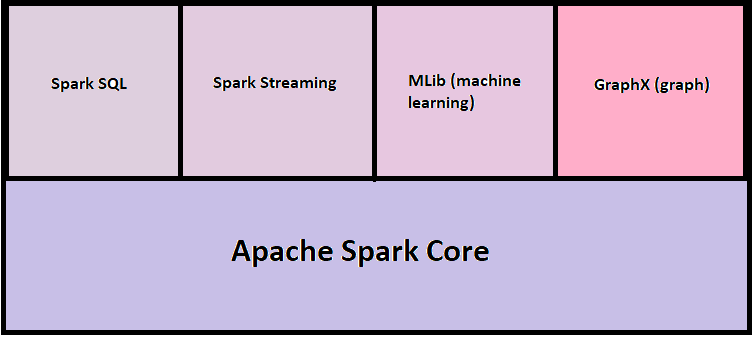
\includegraphics{capitulo2/images/sparkComponentes.png}
		\caption{Componentes que conforman Apache Spark.}
		\label{fig:sparkComponentes}
	\end{center}
\end{figure}

\begin{UClist}
	\UCli \textbf{Spark Core:} Es el núcleo de Spark. Contiene librerías que se utilizan en todos los demás módulos.\\

	\UCli \textbf{Spark SQL:} Módulo para el procesamiento de datos estructurados y semi-estructurados. Esto se conoce como \emph{SchemaRDD}. Este módulo hace posible el uso de lenguaje SQL para hacer consultas.\\

	\UCli \textbf{Spark Streaming:} Este módulo hace posible el procesamiento en tiempo real. Hace posible el flujo de gran cantidad de datos a alta velocidad.\\

	\UCli \textbf{MLib:} Este módulo contiene herramientas y algoritmos muy variados para usar de manera fácil, práctica y escalable al \emph{machine learning}.\\

	\UCli \textbf{GraphX:} Este módulo permite el procesamiento gráfico. No pinta gráficos, sino que realiza operaciones con grafos.\\

\end{UClist}